\chapter{Implementation}\label{sec:implementation}
\section {The original tool}
The original tool is a Graphical Integrated Development Environment called QCADesigner, which is both meant for easing the process of layouting a QCA cells based circuit and for simplyfing the process of simulation and collection of the results. The layout view allows to place on the virtual PCB any number of QCA cell and defining if it is an input, output or fixed one. This discrimination makes it possible for the system to understand of which cells it is meaningful to record the polarization (the output cells) and to which one it is meaningful to assign a value (the input cells). Two different ways of simulating the behaviour of the circuit are implemented: the Coherence Vector and the Bistable engines. 

Both realize the abstract notion of Cellular Automata: the status of every cell at a given instant $t$ strictly depends on its state and on that of its neighborhood at $t-1$. The reason why two engines exist is quite simple: Bistable simulates the behaviour of the circuit from a ``logical'' point of view, meaning that it basically ``switches'' the polarization of every cell based on the polarization of the neighborhood and the current clock in \textsl{just one step}. Coherence Vector, instead, calculates at each instant $t$ the current polarization of the cell and that of its neighborhood and integrates over time the differential equations describing this system in order to make it evolve. Their authors compare and contrast these two engines this way: ``...It is believed that although this approximation [that of Bistable engine] is sufficient to verify the logical functionality of a design it cannot be extended to include valid dynamic simulation; but, as a result of its simplicity this simulation engine is able to simulate a large number of cells very rapidly, and therefore provides a good in-process check of the design. For dynamical simulations refer to the coherence vector simulation. ``. A few number of parameters allow for the customization of the behaviour of both engines in order to make the simulation as accurate and fast as possible. A few rules of thumb are available on the web site of the MiNa Group in order to effectively set some of them.

In the original implementation, moreover, it is possible to look at the evolution of the polarization of every cell during the simulation process.
\section {The bottlenecks of the original implementation}
First of all let's make a basic asymptotic analysis of the implementation of the Coherence Vector algorithm: we have $n$ cells that can have an average of $b$ neighbours. The engine basically runs trough every cell (this goes as $O(n)$) in the design and compute the current polarization based on the polarization of the previous step of all the neighbours (this goes as $O(b)$), and this is done for any possible combination of the inputs (this goes as $O(2^i)$). That is an asymptotic time complexity of $O(2^i*n*b)$  (worst case: $b$=$n-1$) and a space complexity of $O(n*b)$ (only the vector of the polarizations and the vector of neighbors of every cell must be saved, anything else is computed using these values).

Now, the main bottleneck of the original implementation derives from the \textsl{serialization} of the simulation of a system that could be actually evolved \textsl{in parallel}, both with respect to $i$ (eg: one thread per configuration of the inputs) and with respect to $n$ (eg: one thread per cell per iteration). The original simulation of the system in this serial fashion, moreover, introduces some additive error (even though distributable over all cells randomizing the order in which they are simulated at each iteration) due to an overlapping of the writes related to different time instants. 

Our focus is set, in particular, on the Coherence Vector engine. The evidence of the limitations of the bottlenecks, here, are more evident than in Bistable because there is not not even the stabilization phase that would require additional costly synchronization mechanism/convergence criteria at each iteration of the simulation. In Coherence Vector mode the system is always free to evolve.

Before starting talking about the improved version it is good to remember that a number of runs of a set of test circuits has been made with QCADesigner in order to establish the baseline for the evaluation of the progresses (measured in seconds necessary to run the entrire simulation).
\section {Parallelization in CUDA}
\subsection{The approach}
The guiding idea during the parallelization process is: any cell in the system evolves independently with respect to the evolution of the other cells at the same time, but only on the previous state of the machine. Moreover, any input configuration is totally independent on every other possible configuration. In line of principle, this could be approached in one (or both) of these two ways:
\begin{itemize}
\item parallelize with respect to $i$: spread the computation of all the possible $2^i$ configuration on that many threads.
\item parallelize with respect to $n$: spread the computation of all the cells belonging to the same iteration on that many threads.
\end{itemize}
Our choice has been to follow the latter approach, mainly because 
\begin{itemize}
\item major limiting factor of the former approach: it is feasible only for combinatoric circuits; sequential ones still need to consider the variation of the inputs in order to determine their dynamic. Simulating a sequential circuit by means of a single input is practically useless.
\item the ``one cell-one thread'' approach is easy both to figure out and to manage
\item parallelizing with respect to the number of inputs would make the single kernel \textsl{very} complex, disallowing a number of possible optimizations (eg:occupancy improvement, branch divergence)  
\item not the very same actions should be taken for every cell at any moment of the simulation of different inputs; this introduces a hurdle in terms of branch divergence that doesn't allow the GPU to fully exploit its resources
\item suppose to be simulating $k$ configurations of the inputs at a time. The spatial complexity of the algorithm increases by $k$ (which grows exponentially with the number of inputs!).
\end{itemize} 

Moreover, the second approach allows us to better exploit the SIMD principle proper of all CUDA enabled devices because inside the same iteration of the simulation the actions to be carried over any cells are quite the same (and those cells who are not complying with this general scheme don't induce particularly critic divergences in the kernel). This approach allows for the same instructions to be concurrently executed on different data. In our particular case, the code basically does the same actions of the original implementation, apart from the details regarding the proper distribution of the computation among the available resources.

Last but not least, no \textsl{tile-problem} exists (the problem of overlapping adjacent concurrently simulated areas of circuit) because every single cell evolves independently of the effects of the neighbours at the \textsl{same} time $t$.

\subsection{The implementation}
Now, the datils of the implementation.

\begin{figure}[h!]
	\begin{center}$
		\begin{array}{cc}
			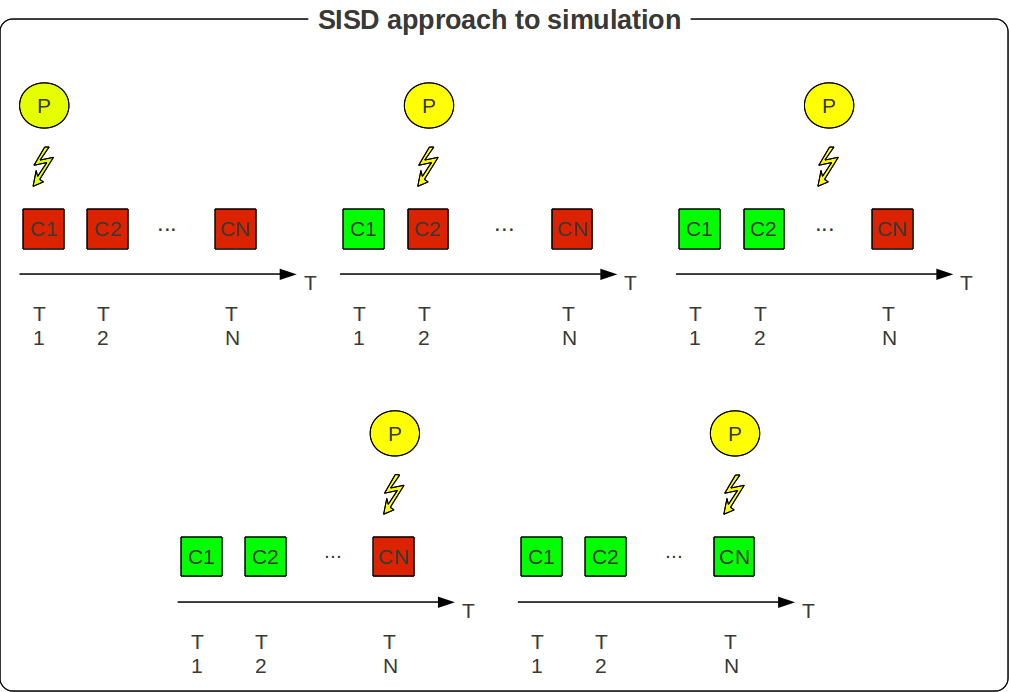
\includegraphics[width=0.5\textwidth]{img/impdetsisd.png} &
			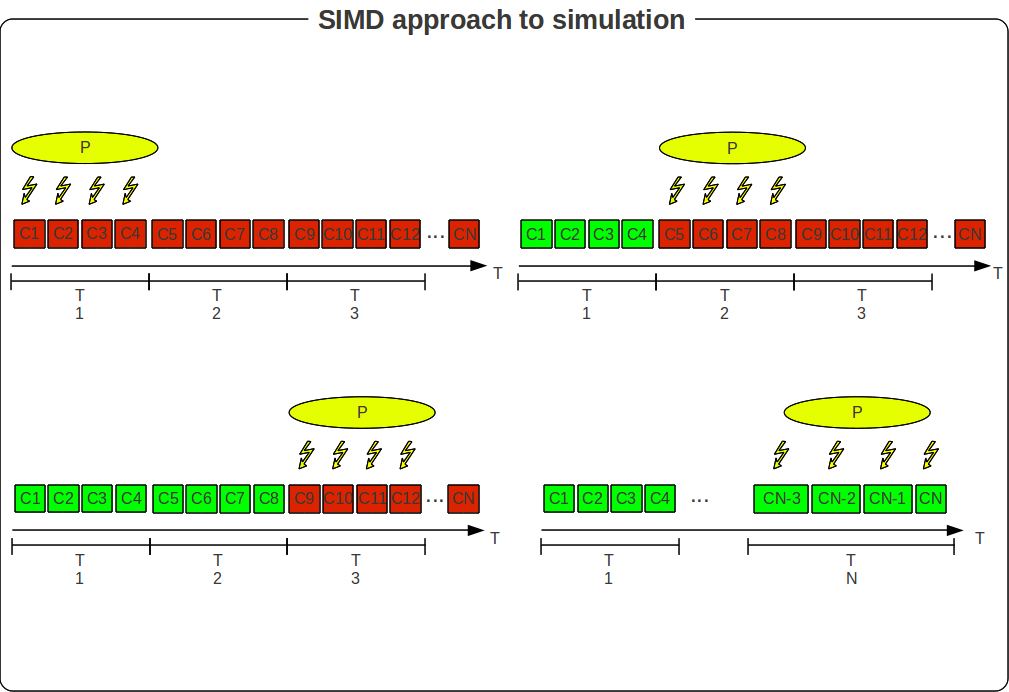
\includegraphics[width=0.5\textwidth]{img/impdetsimd}
		\end{array}$
	\end{center}
	\caption{\label{fig:impdet}In the first approach (SISD) each cell is evolved into the new state \textsl{one at a time}. Observing that any cell inside the same iteration can be evolved \textsl{in parallel} allows us to exploit a SIMD architecture in order to replicate the same instructions over a large number of cells at a time.}
\end{figure}

After an initial phase of parsing the command line commands, the flow of the program goes into Bistable or Coherence Vector engine.

In Coherence Vector mode, three different things happen.

First, all the useful data structures are initialized (for the output, for the parameters of the solver, for the iteration over all the cells into the design, notably). Among the others, some structures we had to implement in order to ease the process of converting the orignal data to CUDA compatible ones. In particular, we extract the following data:
\begin{itemize}
\item \textsl{polariztion vector} the vector of the initial polarization of every cell  (size: $n$)
\item \textsl{neighbour matrix} the unique index associated to every cell is found in this vector in position $i$ if and only if that cell is a neighbour of cell of uinique identifier $i$  (size: $n*b$)
\item \textsl{clock value} a value between 0 to 3 representing the phase of the clock (size: $n$)
\item \textsl{kink energy matrix} the element in position x,y contains the double representing the kink energy between element x and element y, and it is fixed troughout the whole simulation. (size: $n*b$)
\item \textsl{next polarization vector} each element of this matrix represents the evolution of the state of the corresponding cell and is computed by an apposite kernel function (size: $n$)
\end{itemize}
These data are represented in Figure \ref{fig:impdetmem}

\begin{figure}[h!bt]
	\centerline{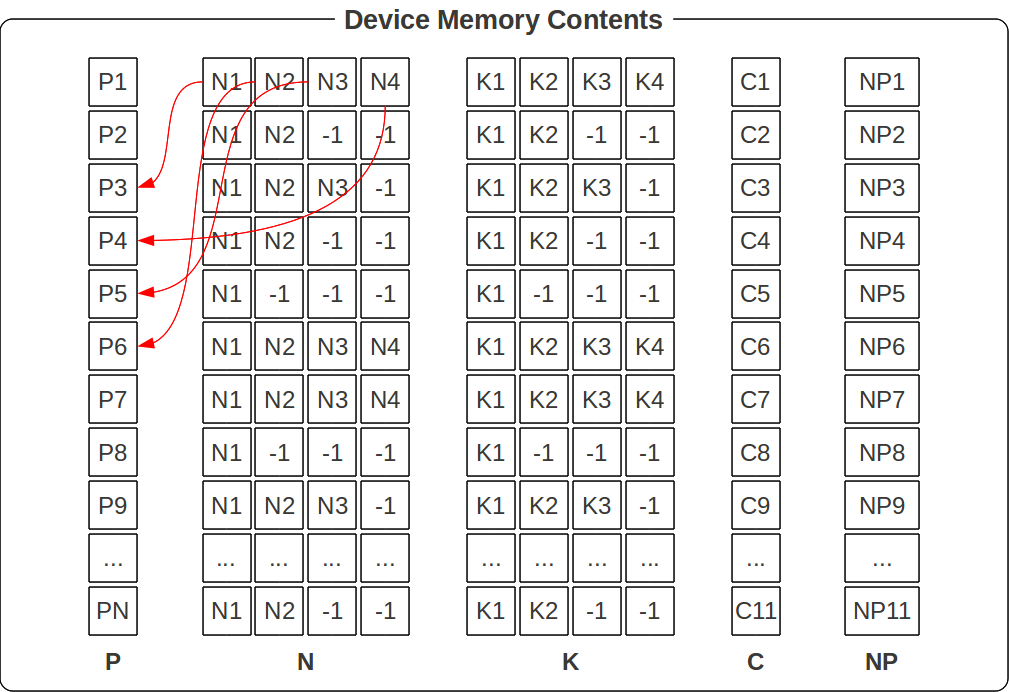
\includegraphics[width=0.8\textwidth]{img/impdetmem.png}}
	\caption{The contents of the memory. \textbf{P} and \textbf{NP} are, respectively, the vector of current polarization and the vector of next/future polarization. \textbf{N} is the matrix containing the ``pointers'' (in red) to the neighboring cells. A $-1$ in any position means that there are no more neighbours. This is because not all the cells must have the same number of neighbors and the matrix must have fixed dimensions while no value can be left unset. \textbf{K} matrix, instead, represent the kink energy that is instaurated between the corresponding neighbouring cells. \textbf{C} vector contains the clock value (the pahse of) for the corresponding cell.}
	\label{fig:impdetmem}
\end{figure}

Second, a number of calls to the framework APIs are made in order to load all the necessary data to the GPU. During this phase the geometry of the blocks of threads is also defined.

Third, the main iteration begins its execution. This loop is executed $f$ times, one for each instant required to completely simulate all the possible combinations of the inputs with the given time sampling (which is indeed a parameter settable via the command line). During each of the $f$ iterations all the $n$ cells in the design are evolved. This is basically the same happening in the serial code with the exception that we are capable of launching \textsl{one thread per cell}, each of which is able to calculate autonomously the evolution of the cell and storing this result in the corresponding cell of the \textbf{NP} vector (refer to Figure \ref{fig:impdetmem}). 

This part of the algorithm is the core of the speedup of our solution. What we do here, in contrast with the SISD approach of the original version of Coherence Vector, is exploiting a SIMD architecture in order to run $T$ (truly parallel) threads computing the evolution of $T$ different cells at once, without compromising the correctness of the simulation.

At the end of each iteration, the \textbf{NP} vector is transferred back from device to host memory and the polarization values written back into the original structures in order to be further treated, for example for saving to the output structures. These steps could have been (partly) done in GPU, but the cost\slash benefit ratio has been estimated too high to be convenient improving this part of the code. After this phase, the iteration goes to instant $t+1$, the polarizations are loaded into device memory and the evolution kernel is launched once again.

Our approcach, moreover, reduces the overall simulation error with respect to the CPU one: in fact, the evolution of the single cell in CPU mode is directly overwritten inside the \textsl{current} state, thus leading to the undesired effect of computing the state of the neighbour of $x$ with a polarization value that is already the future one. This is a limitation known to the MiNa Group who preferred to save execution time (otherwise to be dedicated to costly memory allocations/deallocations) in favour of a slightly more imprecise simulation.

After these improvements, the complexity of the algorithm changes in the following way. From a time perspective we have a theorethical speedup by $T$ running threads; in reality it is slightly less due to the inveitable serializations of the threads concurrently accessing the polarizations of common neighbors in the \textbf{P} vector and only under the assumption that the (time spent loading data to/from device/host)/(time spent simulating the circuit inside the GPU) ratio is negligible. This is similar to what happens with loop unrolling + software pipelining. From a space perspective, instead, we obtain (refer to Figure \ref{fig:impdetmem}) a complexity of $O(3*n+2*n*b)=O(n(3+2*b))$ (worst case: $b=n-1$).
\subsection{Optimizations}
A number of optimizations have been taken into account for improving the overall performance of the program.
\begin{itemize}
\item \textsl{memory hierarchy exploitation} memory in CUDA is higly hierarchical. Global memory is the main and largest memory pool of the device, at the cost of the slowest access speed. For this reason, whenever possible, it has been tried to move data to constant memory (e.g. all the optimization dependent constant values, pre calculated ones etc). No shared memory can be effectively shared between threads because the neighbours of a cell are not necessarily the same neighbours of another thread in the same warp. Other examined solutions comprised more or less huge (read: low speed) transfers of data from host to device memory, impacting at once both on the size of the largest possible simulated circuit and a huge amount of overhead not justified by a proportional in-kernel time. For example, instead of passing the uinique identifiers to the neighboring cells (the \textbf{N} matrix) one could directly pass the \textsl{value} of their polarization, allowing, for example, easier coalescent accesses. Even though, at first, this approach could be positively judged, at a deeper inspection it results in a predictable failure. In fact, every time the iteration ends we are required to exit from the kernel and overwrite the old polarization values with the new ones, thus \textsl{invalidating} the matrix passed just the step before. Our estimate is that a transfer of $n*b$ more doubles (64bit each in CUDA) at each iteration would impose a strong penalty to those circuits that are particulary well suited for simulation in GPU, \textsl{id} est the big ones.
\item \textsl{register usage} registers in CUDA capable devices are a scarce resource that directly and strongly impact the overall performance of a kernel. In fact, the number of threads \textsl{truly} concurrently running depends on how many registers are available inside the streaming multiprocessor to support their execution. Even though it is possible to define what is the optimal geometry of the running blocks by hand, nVidia made available a simple spreadsheet that allows for a fast computation of the optimal parameters for the particular kernel running on the particular system. The term ``occupancy'' in this context refers to the efficiency at exploiting the resources and is defined, more precisely, as the ratio of active warps to the maximum number of warps supported on a multiprocessor of the GPU. Obviously, the higher the occupancy, the higher the active warps, the faster the computation. In order to improve the occupancy factor we developed two different versions of the main kernel, one for each type of integration method employed fo the evolution of the polarization of the cells. This allowed us to reduce at once both the complexity of the single kernel (reducing the number of branches and the total number of instructions) as well as the number of registers required to run them (from 20 to 16, each 64 bits wide).
This is actually the best ppossible solution under a Tesla C1060 (the actual card used for testing purposes), yelding, in fact, a 100\% occupancy rate.
\item \textsl{exploitation of fast\_math} CUDA capable devices do not fully comply to the IEEE754 standard for floating point, double precision operations in that they allow a bigger ulp error for certain operations, in particular for trigonometric ones. In particular, the absolute value of the difference in ulps between a correctly rounded double-precision result and the result returned by the CUDA library function is 2 for cosine and 1 for the hyperbolic tangent. In our code we largely make use of floating point operations, so, by Amdhal's law, it is a good place where to look for improvements. One of those could be the demoting of the double arguments to float ones, in order to exploit the fast\_math mode of the CUDA C math library. In this mode, cosine function and division operation take only one clock cycle to execute, allowing for the highest possible troughput under this architecture. [noi non l'abbiamo ancora provata, potrebbe essere interessante ma nn abbiamo tempo per testarla - la mettiamo? la mettiamo come possibile ma non testata per motivi di tempo?]
\item \textsl{small transfers of data to/from host/device memory} these are by far the slowest possible operations that must be limited as much as possible. Our solution requires the lowest number of transfers among the proposed ones. Profiling of our code yield
\end{itemize}
